\newpage
{\bfseries ҒТАМР 31.23.21}
\hfill {\bfseries \href{https://doi.org/10.58805/kazutb.v.2.23-358}{https://doi.org/10.58805/kazutb.v.2.23-358}}

\sectionwithauthors{Ж.С. Нұрмағанбетов, О.А. Нүркенов, С.Д. Фазылов, А.М. Ибрайбекова, Г. Хабдолда, Б. Әшірбекова}{ЛУПИНИН АЗИДІНІҢ ОРЫНБАСЫЛҒАН АРИЛАЦЕТИЛЕНДЕРМЕН ӨЗАРА ӘРЕКЕТТЕСУЛЕРІ}

\begin{center}
{\bfseries Ж.С. Нұрмағанбетов\textsuperscript{1,2}, О.А. Нүркенов\textsuperscript{1}, С.Д. Фазылов\textsuperscript{1}\envelope, А.М. Ибрайбекова\textsuperscript{2}, Г. Хабдолда\textsuperscript{2}, Б.
Әшірбекова\textsuperscript{2}}

\textsuperscript{1}Қазақстан Республикасының Органикалық синтез жəне
көмір химиясы институты,

Қарағанды, Қазақстан,

\textsuperscript{2}Қарағанды медицина университеті. Қарағанды,
Қазақстан,

\envelope Корреспондент-автор: iosu8990@mail.ru
\end{center}

Мақалада лупинин алкалоидының екіорынбасылған 1\emph{Н}-1,2,3-үшазол
туындылары қатарының синтезі мен құрылымдық ерекшеліктері туралы
зерттеулердің нәтижелері келтірілген. Лупинин алкалоидының химиялық
трансформациясы хинолизин қаңқасының С-1 жағдайда орналасқан
гидроксиметилен тобы бойынша жүзеге асырылды. Реакциялар үш кезеңде әр
түрлі еріткіштерде жүргізілді. Лупининнің метансульфохлоридпен
үшэтиламиннің қатысуымен өзара әрекеттесуі кезінде жоғары шығымдылықпен
лупининнің мезилаты оңай түзілетіні көрсетілді. Осы қосылысты
диметилформамид ерітіндісінде натрий азидімен ары қарай қыздырып өңдеу
нәтижесінде жоғары шығыммен лупинин азидінің түзілуі жүреді. Жаңа
азидтің мыс купоросының сулы және натрий аскорбаты қатысуымен
диметилформамид ерітіндісінде әртүрлі сипаттағы функционалды
орынбасылған ароматты алкиндермен өзара әрекеттесуі кезінде оларға
сәйкес 4-алмастырылған лупининнің үшазолды туындыларының түзілуі мүмкін
екендігі анықталды. Лупининнің үшазолды циклінің негізінде С-4
жағдайында орынбасылған ароматты жаңа туындылары синтезделді.
Синтезделген үшазолдықосылыстардың құрылысы ЯМР \textsuperscript{1}Н
және \textsuperscript{13}С спектрлерін талдау негізінде дәлелденілді.
Жаңа заттардың ЯМР \textsuperscript{13}С спектрлеріндегі сигналдардың
мультиплеттілігі J-модуляция режимінде (JMOD) жазылған спектрлер бойынша
анықталды. Синтезделген қосылыстардың құрылысы сондай-ақ екі өлшемді
COSY (\textsuperscript{1}H-\textsuperscript{1}H) және HMQC
(\textsuperscript{1}H-\textsuperscript{13}C) спектрлерінің деректерімен
зерттелген. ЯМР спектрлердегі химиялық ығысулардың мәндері
\textsuperscript{1}Н және \textsuperscript{13}С сигналдарының
мультиплеттілігі және интегралды қарқындылығы бір өлшемді ЯМР
спектрлерімен анықталды.

{\bfseries Түйін сөздер:} хинолизинді алкалоид, лупинин, азид, ароматты
ацетилендер, үшазолдар, 1,3-екіполярлы циклді қосылу реакциясы.

\begin{center}
{\large\bfseries ВЗАИМОДЕЙСТВИЕ АЗИДА ЛУПИНИНА С ЗАМЕЩЕННЫМИ АРИЛАЦЕТИЛЕНАМИ}

{\bfseries Ж.С. Нурмаганбетов\textsuperscript{1,2}, О.А.
Нуркенов\textsuperscript{1}, С.Д. Фазылов\textsuperscript{1}\envelope, А.М.
Ибрайбекова\textsuperscript{2} ,}

{\bfseries Г. Хабдолда\textsuperscript{1}, Б.
Аширбекова\textsuperscript{2}}

\textsuperscript{1}Институт органического синтеза и углехимии Республики
Казахстан,

Караганда, Казахстан,

\textsuperscript{2}Медицинский университет Караганды. Караганда,
Казахстан,

e-mail: iosu8990@mail.ru
\end{center}

В статье приведены результаты исследований по синтезу и особенностей
строения ряда новых дизамещенных 1\emph{Н}-1,2,3-триазоловых производных
алкалоида лупинина. Химическая трансформация хинолизинового остова в
строении молекулы лупинина осуществлялась по гидроксиметиленовой группе
в положении С-1. Реакции проводились в несколько стадии в среде
различных растворителей. Показано, что при взаимодействии лупинина с
метансульфохлоридом в присутствии триэтиламина в образуется новые
мезилатные производное лупинина. Последующая обработка данного
соединения действием азида натрия в среде диметилформамида при
нагревании проводит к образованию азидпроизводного лупинина с высоким
выходом. Установлено, что при реакции азида с функционально замещенными
ароматическими ацетиленами различной природы в присутствии водного
медного купороса и аскорбата натрия в диметилформамида могут быть
образованы соответствующие 4-замещенные ароматические производные
лупинина. Получены новые производные лупинина, содержащие различные
арильные заместители в положении С-4 триазольного цикла. Строение
полученных соединений установлено на основе анализа спектров ЯМР
\textsuperscript{1}Н и \textsuperscript{13}С. Мультиплетность сигналов
новых соединений в спектрах ЯМР \textsuperscript{13}С определена по
спектрам, записанным в режиме J-модуляции (JMOD). Отнесение сигналов в
спектрах триазоловых соединений проведено с привлечением различных
современных методов корреляционной спектроскопии
\textsuperscript{1}H-\textsuperscript{1}H (COSY), и
\textsuperscript{1}H-\textsuperscript{13}C (HMBC, HSQC). Определены
значения химических сдвигов, мультиплетность и интегральная
интенсивность сигналов \textsuperscript{1}Н и \textsuperscript{13}С в
одномерных спектрах ЯМР.

{\bfseries Ключевые слова}: хинолизиновый алкалоид, лупинин, азид,
ароматические ацетилены, триазолы, реакция 1,3-диполярного
циклоприсоединения.

\begin{center}
{\large\bfseries INTERACTION OF LUPININE AZIDE WITH SUBSTITUTED ARYLACETYLENES}

{\bfseries Zh.S. Nurmaganbetov\textsuperscript{1,2}, O.A.
Nurkenov\textsuperscript{1}, S.D. Fazylov\textsuperscript{1}\envelope, A.M.
Ibraybekova\textsuperscript{2},}

{\bfseries G. Khabdolda\textsuperscript{2}, B.
Аshirbеkоva\textsuperscript{2}}

\textsuperscript{1}Institute of Organic Synthesis and Coal Chemistry of
the Republic of Kazakhstan,

Karaganda, Kazakhstan,

\textsuperscript{2}Medical University of Karaganda. Karaganda,
Kazakhstan,

e-mail: iosu8990@mail.ru
\end{center}

The article presents the results of studies on the synthesis and
structural features of a number of disubstituted
1\emph{H}-1,2,3-triazole derivatives of the lupinine alkaloid. The
chemical transformation of the quinolysin backbone in the structure of
the lupinin molecule was carried out by the hydroxymethylene group at
position C-1. The reactions were carried out in several stages in a
medium of various solvents. It has been shown that when lupinine
interacts with methanesulfochloride in the presence of triethylamine, a
mesylate derivative of lupinine is formed in methylene chloride.
Subsequent treatment of this compound by the action of sodium azide in a
dimethylformamide medium under heating leads to the formation of an
azide derivative of lupinine with a yield of 67\%. It was found that
when azide interacts with functionally substituted aromatic acetylenes
of various natures in the presence of aqueous copper sulfate and sodium
ascorbate, corresponding 4-substituted aromatic triazole derivatives of
lupinine can be formed in dimethylformamide. New 1,2,3-triazole
derivatives of lupinine, containing various aryl substituents at the C-4
position of the triazole ring, have been obtained. The structure of the
obtained compounds was established based on the analysis of the
\textsuperscript{1}H and \textsuperscript{13}C NMR spectra. Multiplicity
of signals of new compounds in the \textsuperscript{13}C NMR spectra was
determined from the spectra recorded in the J-modulation mode (JMOD).
The assignment of signals in the spectra was carried out using various
modern methods of correlation spectroscopy
\textsuperscript{1}H-\textsuperscript{1}H (COZY), and
\textsuperscript{1}H-\textsuperscript{13}C (HMBC, HSQC). The values of
chemical shifts, multiplicity and integral intensity of
\textsuperscript{1}H and \textsuperscript{13}C signals in
one-dimensional NMR spectra are determined.

{\bfseries Keywords:} quinolyzine alkaloid, lupinine, azid, aromatic
acetylenes, triazoles, 1,3-dipolar cycloaddition reaction.

\begin{multicols}{2}
{\bfseries Кіріспе.} Үшазолдардың 1,2,4-туындылары негізінде жаңа тиімді
дәрілік заттарды алудың синтетикалық мүмкіндіктерін соңғы жылдардағы
әдеби деректердің көздерін талдаудан байқауға болады {[}1{]}. Олардың
бірқатар туындылары медициналық тәжірибеде саңырауқұлақ инфекцияларын
(флуконазол, итраконазол, терконазол), вирустық инфекцияларды
(рибавирин, маравирок), психикалық бұзылуларды (тразодон, нефазодон,
альпразолам, триазолам, бротизолам), сүт безі қатерлі ісігін (летрозол,
анастрозол), жүрек-қан тамырлары ауруларын (тиотриазолин, кардиотрил,
трапидил) емдеуге арналған дәрі ретінде қолданылады {[}2{]}. Ғылыми
әдебиеттерде бактерияға қарсы, аналептикалық, жергілікті анестетикалық,
анальгетикалық, қабынуға қарсы, антипиретикалық, гипертензияға қарсы,
гепатопротекторлық, кардиопротекторлық, антиоксидантты, антиагрегантты
және басқа да белсенділік түрлерін көрсететін триазолдардың бірқатар
1,2,4-туындылары белгілі {[}3-5{]}.

Биологиялық белсенді үшазолдардың 1,2,4-туындыларын іздеудің тиімді
бағыты олардың жаңа реагенттермен реакцияларын зерттеу нәтижесінде
белгісіз қосылыстар қатарының пайда болуымен ерекшеленеді {[}6-8{]}.
Реагенттердің бұл түріне мысал ретінде химиялық процестердің
әртүрлілігімен ерекшеленетін хинолизидин қатарының алкалоидтарын
қарастыруға болады {[}9-11{]}. Үшазолды 1,2,4-туындылардың үш таутомерлі
түрде кездесуіне байланысты олардың табиғи құрылымдармен реакцияларын
зерттеу органикалық химия тұрғысынан да, биологиялық белсенді
қосылыстардың жаңа қатарларын синтездеу тұрғысынан да қызығушылық
тудырады. Осылайша, үшазолдардың 1,2,4-туындыларының әр түрлі
алкалоидтармен, атап айтқанда табиғи лупинин алкалоидымен реакцияларын
жүйелі түрде зерттеу, осы негізде биологиялық белсенді қосылыстардың
жаңа топтарын синтездеудің өзіндік әдістерін әзірлеу, сондай-ақ олардың
химиялық және биологиялық қасиеттерін зерттеу өзекті мәселеге жатады.

Фармакологиялық әсерге сәйкес лупинин бактерицидті, шамалы седативті
әсерді, қысқа мерзімді антигельминтикалық және гипотензивті қасиеттерді
байқатады. Оның белгілі туындыларының ішінде эфирлері ең көп зерттелген,
олар түрлі тымауларға, ісікке қарсы және гепатопротекторлық
белсенділікке ие. Бірқатар лупинин эфирлері жергілікті анестетикалық
әсерді, сондай-ақ көкжөтелге қарсы және холинестераздарға белсенділікті
көрсетті {[}12{]}. Хлорлы лупинан, күкіртті лупинан және цианды лупинан
негізінде психикалық және моторлық бұзылулардың патогенезіне қатысатын
орталық жүйке жүйесінің \emph{сигма}-рецепторлары үшін тиімді лигандалар
ретінде лупинин алкалоидының әртүрлі туындылар қатары синтезделді
{[}13-15{]}. Сондықтан лупининге және оның жаңа туындыларына деген
қызығушылық шексіз. Лупининнің құрылысын түрлендірудің аз зерттелген
және тиімді бағыттарының бірі оның ықтимал биобелсенді үшазолды
туындыларын алу болып табылады. Осылайша, лупинин алкалоидының ықтимал
биобелсенді үшазол туындыларын түрлендірудің ыңғайлы әдістерін іздестіру
және өңдеу биоорганикалық химия мен фармакологияда маңызды өзекті
мәселенің бірі деп атауға болады.

{\bfseries Материалдар және әдістер.} Жаңа заттардың ИҚ спектрлері
Vector-22 фурье спектрометрінде КВг таблеткаларында жазылған. ЯМР
\textsuperscript{1}H- және \textsuperscript{13}C-спектрлері Bruker
AV-400 (400 және 101 МГц) және Bruker DRX-500 (500 және 125 МГц)
спектрометрлерінде тіркелген. Синтезделген қосылыстардың спектрлері
CDCl\textsubscript{3} жазылды, оның қалдық сигналдары
(δ\textsubscript{С}=76.9 м.ү.) және (δ\textsubscript{Н}=7.24 м.ү.) ішкі
стандарт ретінде пайдаланылды. Алынған қосылыстардың құрылымы ЯМР
\textsuperscript{1}Н- және \textsuperscript{13}С-спектрлерін талдау
негізінде дәлелденілді, ЯМР \textsuperscript{13}С-спектрлеріндегі
сигналдардың мультиплеттілігі J-модуляция режимінде (JMOD) жазылған
спектрлер бойынша анықталды. Хинолизин қанқасы үшін
\textsuperscript{1}H-\textsuperscript{1}H (COSY) және
\textsuperscript{1}H-\textsuperscript{13}C (HMBC, HSQC) спектрлердегі
сигналдардың ерекшеліктері әр түрлі корреляциялық спектроскопиядағы
әдеби деректерді пайдалану арқылы жүзеге асырылды. Спектрлерді сараптау
кезінде келтірілген негізгі атомдардың нөмірленуі липинин молекуласының
({\bfseries 1)} құрылымы бойынша қолданылды. Меншікті айналу мәндері PolAAr
3005 поляриметрінде түсірілді. Жоғары ажыратымдылықтағы масс-спектрлер
DFS ThermoScientific масс-спектрометрінде жазылған (буландырғыш
температурасы 200-250°С, ЭУ иондануы, 70 эВ). Балқу температурасы
Mettler Toledo FP900 терможүйесінде анықталды. Реакциялардың жүру
барысын бақылау Sorbfil UV-254 пластиналарында жұқақабатты хроматография
(ЖҚХ) әдісімен әртүрлі жүйелерді қолдана отырып жүзеге асырылады:
трихлорметан, трихлорметан-этил спирті, 10:1. Жұқа қабатты
хроматографияның көрінісі йод камерасында және ультракүлгін сәуледе
бақыланды. Реакция өнімдері қайта кристалдану немесе Acros силикагелінде
(0.035--0.240 мм) бағаналы хроматография арқылы таза түрде бөлінген,
элюенті еріткіштер ретінде: трихлорметан; трихлорметан-этил спирті,
100:1→10:1) қолданылды.

{\bfseries Функционалды орынбасылған үшазолдардың 5a-f синтезі (жалпы
әдіс).} 6 мл ДМФА еріткішінде 0.29 г (1.5 ммоль) лупининнің азиді
{\bfseries 3} ерітіліп, функционалды орынбасылған ароматты ацетилендердің
{\bfseries 4а-f} 1.35 ммоль, мыс купоросы 0.034 г (0.135 ммоль) және
натрийдің аскорбаты 0.026 г (0.135 ммоль) қосылып 75°С температурада
қыздыру жағдайында 6-8 сағат араластырылды (реакция жүру барысы ЖҚХ
әдісімен бақыланды). Салқындату жағдайында түзілген тұнба сүзіліп
алынды, содан кейін гексан еріткішімен жуылып, кептіріліп, {\bfseries 5а-f}
үшазолдары алынды. Түзілген {\bfseries 5а-f} үшазолдар препаративті таза
алу мақсатында флеш бағанасында силикагель сорбентімен
хроматографияланды (элюент: трихлорметан, трихлорметан:этил спирті,
100:1→10:1).

{\bfseries (1\emph{S},9a\emph{R})-1-{[}4-Фенил-1\emph{Н}-1,2,3-үшазол-1-ил)метил{]}октагидро-1\emph{Н}-хинолизин
5а.}

Шығымы 0.3 г (75\%). Ақ ұнтақты зат, балқу т. 196-197°С.
{[}α{]}\textsubscript{D}-19.7 (\emph{с} 0.8, трихлорметан).

ИҚ спектр (KBr), ν, см\textsuperscript{-1}: 694, 766, 835, 1441, 1466,
1485, 1505, 1612, 3120 (С=С, С=N), 2763, 2804 (хинолизидинді сақина).

ЯМР \textsuperscript{1}Н спектрі (400 МГц, CDCl\textsubscript{3}), δ,
м.ү. (J, Гц): 1.17-1.40 (3Н, м., Н-2а, 2e,8a); 1.41-1.64 (5Н, м.,
Н-8е,9a,9e,3а,7а); 1.73-1.92 (2Н, м., Н-3е,7е); 1.94-2.04 (2Н, м., Н-4а,
Н-6а); 2.06-2.11 (1Н, м., Н-9а), 2.21-2.25 (1Н, м., Н-1); 2.82-2.88 (2Н,
м., Н-4е,6е); 4.55 (1Н, д.д., J=13.6, J = 5.8, Н-10); 4.62 (1Н, д.д.,
J=13.6, J=12.0, Н-10); 7.29 (1Н, т., J=7.6, Н-4ʹʹ); 7.39 (д.д., 2Н,
J=7.4, 7.6, Н-3ʹʹ, Н-5ʹʹ); 7.70 (1Н, с., Н-5ʹ), 7.80 (2Н, д., J=7.4,
Н-2ʹʹ, Н-6ʹʹ).

ЯМР \textsuperscript{13}C спектрі (125 МГц, CDCl\textsubscript{3}), δ,
м.ү.: 20.5 (С-3); 24.7 (С-7); 25.3 (С-8); 26.3 (С-2); 29.5 (С-9); 39.1
(С-1); 48.5 (С-10); 56.9 (С-4); 57.1 (С-6); 64.2 (С-9а); 120.0 (С-5ʹ);
125.6 (2С, \emph{о}-С\textsubscript{6}Н\textsubscript{5}); 127.9 (С,
\emph{р-}С\textsubscript{6}Н\textsubscript{5}); 128.7 (2С,
\emph{m}-С\textsubscript{6}Н\textsubscript{5}); 130.7 (С,
С\textsubscript{6}Н\textsubscript{5}); 147.4 (С-4ʹ).

Масс-спектр, m/z (\%): 298 (1), 297 (8), 296 (38), 152 (42), 151 (100),
150 (59), 138 (22), 137 (11), 136 (32), 116 (16), 111 (24), 110 (19), 96
(19), 83 (36), 41 (36). Табылғаны, \emph{m}/\emph{z}: 296.1995
{[}M{]}\textsuperscript{+}.
C\textsubscript{18}H\textsubscript{24}N\textsubscript{4}. Есептелгені,
\emph{m}/\emph{z}: 296.19.

{\bfseries (1\emph{S},9a\emph{R})-1-\{{[}4-(4-Этилфенил)-1\emph{Н}-1,2,3-үшазол-1-ил{]}метил\}октагидро-1\emph{Н}-хинолизин
5b.}

Шығымы 0.41 г (90\%). Ақ ұнтақты зат, балқу т. 188-190°С.
{[}α{]}\textsubscript{D}-16.8 (\emph{с} 1.0, трихлорметан).

ИҚ спектр (KBr), ν, см\textsuperscript{-1}: 723, 750, 831, 1444, 1458,
1498, 1560, 3103 (С=С, С=N); 2763, 2807 (хинолизидинді сақина).

ЯМР \textsuperscript{1}Н спектрі (400 МГц, CDCl\textsubscript{3}), δ,
м.ү. (J, Гц): 1.16 (3Н, т., J=7.2, СН\textsubscript{3}); 1.19-1.40 (3Н,
м., Н-2а,2e,8a); 1.41-1.65 (5Н, м., Н-8е,9a,9e,3а,7а); 1.74-1.90 (2Н,
м., Н-3е,7е); 1.91-2.08 (2Н, м., Н-4а,6а); 2.05-2.11 (1Н, м., Н-9а),
2.21-2.26 (1H, м., Н-1); 2.65 (2Н, кв., J=7.2, CH\textsubscript{2}),
2.82-2.88 (2Н, м., Н-4е,6е); 4.54-4.65 (2Н, м., Н-10); 7.24 (2Н, д.,
J=7.8, Н-2ʹʹ, Н-6ʹʹ); 7.67 (1Н, с., Н-5ʹ); 7.73 (2Н, д., J=7.8, H-3ʹʹ,
Н-5ʹʹ).

ЯМР \textsuperscript{13}C спектрі (101 МГц, CDCl\textsubscript{3}), δ,
м.ү.: 15.6 (CH\textsubscript{3}); 20.7 (С-3); 24.9 (С-7); 25.6 (С-8);
26.3 (С-2); 28.7 (CH\textsubscript{2}Me); 29.8 (С-9); 39.2 (С-1); 48.6
(С-10); 57.1 (С-4); 57.3 (С-6); 64.4 (С-9а); 119.9 (С-5ʹ); 125.6 (С-2ʹʹ,
С-6ʹʹ); 128.2 (С-1ʹʹ); 128.3 (С-3ʹʹ, С-5ʹʹ); 144.3 (С-4ʹʹ); 147.6
(С-4ʹ).

Масс-спектрі, m/z (\%): 325 (4), 324 (17), 231 (11), 152 (19), 151 (53),
150 (32), 136 (29), 135 (28), 122 (43), 121 (74), 120 (37), 105 (71), 91
(21), 70 (100), 69 (70). Табылғаны, \emph{m}/\emph{z}: 324.2306
{[}M{]}\textsuperscript{+}.
C\textsubscript{20}H\textsubscript{28}N\textsubscript{4}. Есептелгені,
\emph{m}/\emph{z}: 324.23.

{\bfseries (1\emph{R},9a\emph{S})-1-\{{[}4-(4-Фторфенил)-1\emph{Н}-1,2,3-үшазол-1-ил{]}метил\}октагидро-1\emph{Н}-хинолизин
5c.}

Шығымы 0.32 г (76\%). Ақ ұнтақты зат, балқу т. 195-198°С.
{[}α{]}\textsubscript{D}-17.5 (\emph{с} 1.0, трихлорметан).

ИҚ спектрі (KBr), ν, см\textsuperscript{-1}: 779, 815, 835 1462, 1497,
1558, 1610, 3105, 3126 (С=С, С=N); 1108, 1126, 1157, 1223 (С-F); 2765,
2808 (хинолизидинді сақина).

ЯМР \textsuperscript{1}Н спектрі (400 МГц, CDCl\textsubscript{3}), δ,
м.ү. (J, Гц): 1.18-1.40 (3Н, м., Н-2а,2e,8a); 1.40-1.64 (м., 5Н,
Н-8е,9a,9e,3а,7а); 1.72-1.90 (2Н, м., Н-3е,7е); 1.93-2.01 (2Н, м.,
Н-4а,6а); 2.05-2.08 (1Н, м., Н-9а), 2.21-2.27 (1H, м., Н-1); 2.82-2.88
(2Н, м., Н-4е,6е); 4.54 (1Н, д.д., J=13.8, J=5.6, Н-10); 4.63 (1Н, д.д.,
J=13.8, J=11.4, Н-10); 7.07 (2Н, м., Н-3ʹʹ, Н-5ʹʹ); 7.65 (1Н, с., Н-5ʹ);
7.77 (2Н, м., H-2ʹʹ, Н-6ʹʹ).

ЯМР \textsuperscript{13}C спектрі (101 МГц, CDCl\textsubscript{3}), δ,
м.ү.: 20.4 (С-3); 24.7 (С-7); 25.4 (С-8); 26.1 (С-2); 29.7 (С-9); 39.0
(С-1); 48.5 (С-10); 56.9 (С-4); 57.1 (С-6); 64.2 (С-9а); 115.6 (д.,
\textsuperscript{2}J\textsubscript{CF}=21.7, С-3ʹʹ, С-5ʹʹ); 119.8
(С-5ʹ); 126.8 (д., \textsuperscript{4}J\textsubscript{CF}=3.2, С-1ʹʹ);
127.2 (д., \textsuperscript{3}J\textsubscript{CF}=8.2, С-2ʹʹ, С-6ʹʹ);
146.5(С-4ʹ); 162.4 (д., \textsuperscript{1}J\textsubscript{CF}=247.5,
С-4ʹʹ).

Масс-спектрі, m/z (\%): 316 (1), 315 (9), 314 (44), 152 (40), 151 (100),
150 (58), 138 (18), 137 (11), 136 (38), 111 (19), 96 (15), 83 (25).
Табылғаны, \emph{m}/\emph{z}: 314.1899 {[}M{]}\textsuperscript{+}.
C\textsubscript{18}H\textsubscript{23}N\textsubscript{4}F. Есептелгені,
\emph{m}/\emph{z}: 314.19.

{\bfseries (1\emph{S},9a\emph{R})-1-(\{4-{[}4-Ацетиламино-3 - (этоксикарбонил) фенил{]}-1\emph{Н}-1,2,3-триазол-1-ил\}метил)октагидро-1\emph{Н}-хинолизин
5d.}

Шығымы 0.5 г (87\%). Ақ ұнтақ зат, балқу т. 157-159°С,
{[}α{]}\textsubscript{D}-9.3 (с 0.8, трихлорметан).

ИҚ спектрі (KBr), ν, см\textsuperscript{-1}: 792, 835, 1443, 1469, 1517,
1597, 3126 (С=С, С=N); 1089, 1230, 1295 (O-С-О);1680 (HN-С=О), 1707
(O-С=О), 2682, 2763, 2808 (хинолизидинді сақина), 3261 (NH).

ЯМР \textsuperscript{1}Н спектрі (400 МГц, CDCl\textsubscript{3}), δ,
м.ү. (J, Гц): 1.18-1.37 (3Н, м., Н-2а,2e,8a); 1.40 (3Н, т., J=7.2,
СН\textsubscript{3}); 1.43-1.63 (5Н, м., Н-8е,9a,9e,3а,7а); 1.73-1.92
(2Н, м., Н-3е,7е); 1.94-2.02 (2Н, м., Н-4а,6а); 2.06-2.11 (1Н, м.,
Н-9а), 2.22 (3Н, с., СН\textsubscript{3}-NH); 2.25-2.30 (1H, м., Н-1);
2.82-2.86 (2Н, м., Н-4е,6е); 4.38 (2Н, кв., J=7.2,
ОСН\textsubscript{2}); 4.57 (1Н, д.д., J=13.7, J=5.5, Н-10); 4.62 (1Н,
д.д., J=13.7, J=11.0, Н-10); 7.71 (1Н, с., Н-5ʹ); 7.86 (1Н, д.д., J=8.8,
J=2.0, Н-6ʹʹ); 8.55 (1Н, д., J=2.0, Н-2ʹʹ); 8.73 (1Н, д., J=8.8, Н-5ʹʹ);
11.13 (1Н, с., NH).

ЯМР \textsuperscript{13}C спектрі (101 МГц, CDCl\textsubscript{3}), δ,
м.ү.: 14.1 (СН\textsubscript{3}); 20.4 (С-3); 24.7 (С-7); 25.3 (С-8);
26.1 (С-2); 25.4 (NСН\textsubscript{3}); 29.6 (С-9); 39.1 (С-1); 48.6
(С-10); 56.8 (С-4); 57.1 (С-6); 61.5 (ОСН\textsubscript{2}); 64.2
(С-9а); 115.4 (С-3ʹʹ); 119.8 (С-5ʹ); 120.4 (C-5ʹʹ); 124.9 (C-1ʹʹ); 127.7
(C-2ʹʹ); 131.4 (C-6ʹʹ); 141.1 (С-4ʹʹ); 146.3 (С-4ʹ); 168.1 (C=O эфир);
168.9 (С=О амид).

Масс-спектрі, m/z (\%): 427 (2), 426 (13), 425 (44), 411 (15), 152 (44),
151 (100), 150 (56), 136 (32), 83 (21), 43 (28). Табылғаны, m/z:
425.2420 {[}M{]}\textsuperscript{+}.
C\textsubscript{23}H\textsubscript{31}N\textsubscript{5}О\textsubscript{3}.
Есептелгені, m/z: 425.24.

{\bfseries (1\emph{S},9a\emph{R})-1-\{{[}4-(3,4,5-үшметоксифенил)-1\emph{H}-1,2,3-үшазол-1-ил{]}метил\}октагидро-
1\emph{H}-хинолизин 5e.}

Шығымы 0.2 г (72\%). Ақ кристалдар, балқу т. 143-145°С.
{[}α{]}\textsubscript{D}-13.6 (\emph{с} 1.6, трихлорметан).

ИҚ спектрі (KBr), ν, см\textsuperscript{-1}: 779, 827, 860, 1467, 1500,
1585, 1639, 3110 (С=С, С=N); 1006, 1099, 1128, 1234 (С-О); 2736, 2765,
2798 (хинолизидинді сақина).

ЯМР \textsuperscript{1}Н спектрі (400 МГц, CDCl\textsubscript{3}), δ,
м.ү. (\emph{J}, Гц): 1.21-1.39 (3Н, м.,
Н-2\emph{а},2\emph{e},8\emph{a}); 1.43-1.64 (5Н, м.,
Н-8\emph{е},9\emph{a},9\emph{e},3\emph{а},7\emph{а}); 1.74-1.90 (2Н, м.,
Н-3\emph{е},7\emph{е}); 1.95-2.09 (2Н, м., Н-4\emph{а},6\emph{а});
2.12-2.17 (1Н, м., Н-9\emph{а}), 2.29-2.34 (1H, м., Н-1); 2.79-2.94 (2Н,
м., Н-4\emph{е},6\emph{е}); 3.84 (C-4ʹʹ тегі 3Н, с.,
OСН\textsubscript{3}); 3.91 (C-3ʹʹ, С-5ʹʹ тегі 6Н, с.,
2×OСН\textsubscript{3}); 4.58 (1Н, д.д., \emph{J}=13.9, \emph{J}=6.0,
Н-10); 4.62 (1Н, д.д., \emph{J}=13.9, \emph{J}=11.2, Н-10); 7.06 (2Н,
с., Н-2ʹʹ, Н-6ʹʹ); 7.71 (1Н, с., Н-5ʹ). \hl{}

ЯМР \textsuperscript{13}C спектрі (125 МГц, CDCl\textsubscript{3}), δ,
м.ү.: 20.4 (С-3); 24.6 (С-8); 25.3 (С-7); 26.1 (С-2); 29.6 (С-9); 39.0
(С-1); 48.5 (С-10); 56.1 (2×OСH\textsubscript{3}); 57.1 (С-4, С-6); 60.8
(ОСН\textsubscript{3}); 64.1 (С-9а); 102.6 (С-2ʹʹ, С-6ʹʹ); 119.9 (С-5ʹ);
126.2 (C-1ʹʹ); 137.9 (С-4ʹʹ); 147.3 (С-4ʹ); 153.4 (C-3ʹʹ, С-5ʹʹ).

Масс-спектрі, m/z (\%): 387 (8), 386 (29), 358 (7), 343 (8), 206 (11),
192 (11), 177 (12), 152 (53), 151 (100), 150 (83), 137 (27), 136 (81),
110 (20), 83 (35), 41 (28). Табылғаны, \emph{m}/\emph{z}: 386.2308
{[}M{]}\textsuperscript{+}.
C\textsubscript{21}H\textsubscript{30}N\textsubscript{4}О\textsubscript{3}.
Есептелгені, \emph{m}/\emph{z}: 386.23.

{\bfseries 1-\{{[}4-(4-(Бензилокси)-3-метоксифенил{]}-1\emph{H}-1,2,3-үшазол-1-ил\}метил)
октагидро-1\emph{H}-хинолизин 5f.}

Шығымы 0.45 г (69\%). Ақ ұнтақты зат, балқу т. 152-155°С.
{[}α{]}\textsubscript{D}-15.1 (\emph{с} 1.2, трихлорметан). \hl{}

ИҚ спектрі, ν, см\textsuperscript{--1}: 694, 740, 790, 812, 846, 1452,
1466, 1504, 1585, 1610, 3090 (С=С, С=N); 1001, 1036, 1132, 1222, 1232
(С-О); 2759, 2802 (хинолизидинді сақина).

ЯМР \textsuperscript{1}Н спектрі (500 МГц, CDCl\textsubscript{3}), δ,
м.ү. (\emph{J}, Гц): 1.18-1.29 (3Н, м.,
Н-2\emph{а},2\emph{e},8\emph{a}); 1.45-1.65 (5Н, м.,
Н-8\emph{е},9\emph{a},9\emph{e},3\emph{а},7\emph{а}); 1.77-1.88 (2Н, м.,
Н-3\emph{е},7\emph{е}); 1.91-2.06 (2Н, м., Н-4\emph{а},6\emph{а});
2.10-2.18 (1Н, м., Н-9\emph{а}), 2.22-2.27 (1H, м., Н-1); 2.80-2.88 (2Н,
м., Н-4\emph{е},6\emph{е}); 3.95 (C-3ʹʹ тегі 3Н, с.,
OСН\textsubscript{3}); 4.55 (1Н, д.д., \emph{J}=13.8, \emph{J}=5.5,
Н-10); 4.61 (1Н, д.д., \emph{J}=13.8, \emph{J}=12.1, Н-10); 5.16 (2Н,
с., ОСН\textsubscript{2}); 7.86 (1Н, д., \emph{J}=8.3, Н-5ʹʹ); 8.16 (1Н,
д.д., \emph{J}=8.3, \emph{J}=2.0, Н-6ʹʹ); 7.26-7.30 (1Н, м.,
С\textsubscript{6}Н\textsubscript{5}, Н-\emph{р}); 7.31-7.37 (2Н, м.,
С\textsubscript{6}Н\textsubscript{5}, Н-\emph{m}); 7.38-7.44 (1Н, м.,
С\textsubscript{6}Н\textsubscript{5}, Н-\emph{о}); 7.50 (1Н, д.,
\emph{J}=2.0, H-2ʹʹ); 7.62 (1Н, с., Н-5ʹ).

ЯМР \textsuperscript{13}C спектрі (125 МГц, CDCl\textsubscript{3}), δ,
м.ү.: 20.5 (С-3); 24.7 (С-8); 25.3 (С-7); 26.1 (С-2); 29.5 (С-9); 39.1
(С-1); 48.5 (С-10); 55.9 (OСН\textsubscript{3}); 56.7 (С-4); 57.1 (С-6);
64.2 (С-9а); 70.9 (ОСН\textsubscript{2}); 109.3 (C-2ʹʹ); 114.1 (C-5ʹʹ);
117.9 (С-6ʹʹ); 119.5 (С-5ʹ); 124.2 (C-1ʹʹ); 127.2 (C-2ʹʹʹ, С-6ʹʹʹ);
127.7 (C-4ʹʹʹ); 128.4 (С-3ʹʹʹ, С-5ʹʹʹ); 136.9 (С-1ʹʹʹ); 147.3 (C-4ʹ);
147.9 (С=4ʹʹ); 149.9 (С-3ʹʹ).

Масс-спектрі, m/z (\%): 434 (2), 433 (12), 432 (41), 313 (18), 258 (15),
152 (50), 151 (52), 150 (38), 136 (17), 91 (100). Табылғаны,
\emph{m}/\emph{z}: 432.2519 {[}M{]}\textsuperscript{+}.
C\textsubscript{26}H\textsubscript{32}N\textsubscript{4}О\textsubscript{2}.
Есептелгені, \emph{m}/\emph{z}: 432.25.
\end{multicols}

\begin{figure}[H]
	\centering
	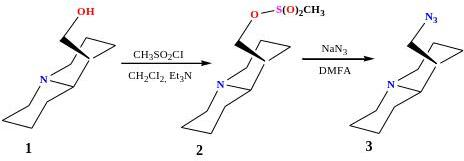
\includegraphics[width=0.6\textwidth]{assets/1011}
	\caption*{}
\end{figure}

\begin{multicols}{2}
{\bfseries Нәтижелер және талқылау.} Бұл жұмыста лупининнің азиді
{\bfseries 3} негізінде құрамында орынбасылған 1,2,3-үшазолды фрагменттері
бар ықтимал биологиялық белсенді қосылыстарының алыну жолдарын
сипаттаймыз. Лупинин азидінің {\bfseries 3} синтезделу жолы {[}16,17{]}
ғылыми әдебиеттерде зерттеліп баяндалған. Бұл реакция 2 сатыды
жүргізілді: 1-ші сатыда мақсатты өнімдер {\bfseries 2}
(СH\textsubscript{3}SO\textsubscript{2}CI ерітіндісінде) және {\bfseries 3}
(ДМФА ерітіндісінде) 93.2 және 67\% шығыммен реакциялық ортадан бөлініп
алынды.

Екінші сатыда лупинин азидінің {\bfseries 3} функционалды орынбасылған
ароматты ацетилендермен {[}фенилацетилен {\bfseries 4a},
4-этилфенилацетилен {\bfseries 4b}, 4-фторфенилацетилен {\bfseries 4c},
5-(этинил)этилантранилат {\bfseries 4d}, 3,4,5-триметоксифенилацетилен
{\bfseries 4e}, 4-бензилокси-3-метоксифенилацетилен {\bfseries 4f}{]} өзара
әрекеттесулері ДМФА ортасында мыс купоросы және натрийдің аскорбаты
қатысында 75°С температурада қыздыру арқылы жүзеге асырылды. Бұл реакция
Сu\textsuperscript{1} катализаторлық әсерімен 1,3-диполяры қосылу
механизмі бойынша жүреді:
\end{multicols}

\begin{figure}[H]
	\centering
	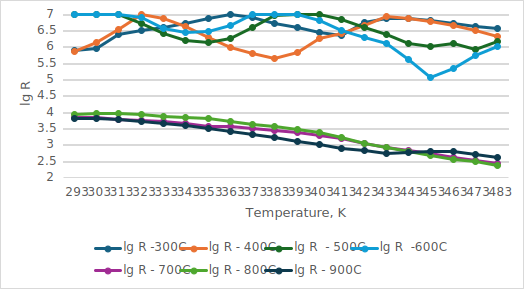
\includegraphics[width=0.6\textwidth]{assets/1012}
	\caption*{}
\end{figure}

\begin{figure}[H]
	\centering
	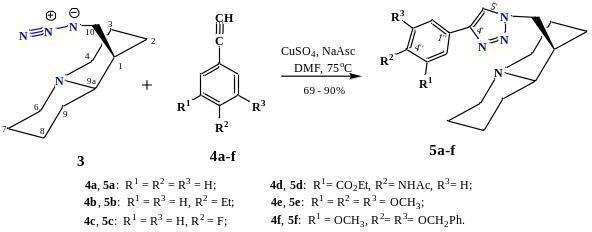
\includegraphics[width=0.6\textwidth]{assets/1013}
	\caption*{}
\end{figure}

\begin{multicols}{2}
Реакция жүру барысы ЖҚХ әдісімен бақыланды. Нәтижесінде бағаналы
хроматография әдісімен құрамында 1,2,3-үшазол циклінің С-4 жағдайындағы
арил-орынбасылған лупининнің үшазолды туындылары ({\bfseries 5а-f})
(шығымдары 69-90\%) таза түрде бөлініп алынды.

Синтезделген қосылыстардың құрамы мен құрылымы ИҚ-, ЯМР
\textsuperscript{1}Н- және \textsuperscript{13}С- спектроскопия және
масс-спектрометрия әдістерімен дәлелденілді. Лупинин азидінің {\bfseries 3}
құрылысында орынбасылған N\textsubscript{3-}тобының болуы ИҚ спектрінің
мәлімдемелерімен анықталды (2096 см\textsuperscript{-1} аймағында азид
тобының валенттік тербелістеріне сәйкес келетін қарқынды сіңіру жолағы
байқалды).

Синтезделген 1,2,3-үшазолды қосылыстардың ЯМР \textsuperscript{1}Н- және
\textsuperscript{13}C-спектрлерінде хинолизин қаңқасына тән және тиісті
орынбасылған фунционалды топтарға қатысты сигналдар жиынтығы кездеседі.
Күшті өріс аймағында (δ 1.17-1.70 м.ү.) интегралдық қарқындылығы 8Н
болатын кең мультиплеттік сигналдар орналасқан, олардың құрамына осьтік
және экваторлық бағыттағы лупинин қаңқасының протондары
(Н-2\emph{a},\emph{e},8\emph{a},\emph{e},9\emph{a},\emph{e},3\emph{a},7\emph{a})
кіреді. Мультиплет сигналы (δ 1.70-1.92 м.ү.) экваторлық бағытталған
H-3,7 протондарына қатысты. Әрі қарай 4,6 (δ 1.88-2.08 м.ү.) аксиальді
протондар, 9а (δ 2.05-2.18 м.ү) түйіндік протондар және С-1 (δ 2.18-2.30
м.ү) протондары резонанс тудырады. 4,6 Экваторлық бағыттағы протондар (δ
2.80-2.88 м.ү.) аймақтағы мультиплетпен ұсынылған. Н-10 метилен тобының
протондары δ 4.51-4.65 м.ү. аймағында екі дублет-дублет түрінде
резонанстық жағдайға әкеледі. {\bfseries 5a-f} Қосылыстардың ЯМР
\textsuperscript{1}H спектріндегі түзілген 1,2,3-үшазолдық циклдардың
протонына δ 7.37--7.71 м.ү. аймағында орналасқан синглетті сигнал жауап
береді. ЯМР \textsuperscript{13}C спектріндегі үшазол циклінің көміртегі
атомдары сәйкесінше 119.3--122.4 м.ү. (С-5) және 146.2--156.8 м.ү. (С-4)
дублет және синглет түрінде байқалады (спектрлер JMOD режимінде
жазылды). Бұл мәлімдемелер СuAС реакциялар нәтижесінде 1,4-орынбасылған
1\emph{H}-1,2,3-үшазолдардың түзілуін растайды {[}18,19{]}.

Барлық қосылыстардың масс-спектрлерінде әртүрлі қарқындылықтағы
молекулалық иондардың шыңдары кездеседі. Барлық синтезделген үшазолды
туындылардың {\bfseries 5а-f} спектрлерінде молекуланың хинолизидинді
қаңқасының С-10 атомы арқылы бөлінуіне сәйкес келетін
С\textsubscript{10}H\textsubscript{17}N (150-151 ш.б.) фрагментті
иондарының шыңдары сипатталған.

{\bfseries Қорытынды.} Мақалада С-10 атомы бойынша лупинин алкалоидының
құрылымын түрлендірудің оңтайлы шарттары ұсынылды және жасалынды, оның
жоғары өнімділігі бар ықтимал биобелсенді 1,2,3-үшазол туындылары
синтезделді. Соңғы үшазол өнімдерін алу екі кезеңде жүзеге асырылды:
аралық лупинин азидінің синтезі және оның 1,3-екіполярлы
{[}3+2{]}-әртүрлі алкиндерге тұйықты қосылуы. Реакциялар ДМФА
еріткішінде мыс сульфаты және натрий аскорбатының қатысуымен жүргізілді.
Лупинин алкалоидының жаңа синтезделіп алынған 1,2,3-үшазолды фрагменті
бар туындылары биологиялық белсенді субстраттың қосымша
лиганд-рецепторлық өзара әрекеттесуін қамтамасыз ете алады және алынған
субстраттың биологиялық әсерінің селективтілігін өзгертеді. Синтезделген
жаңа қосылыстардың құрылыстары ЯМР \textsuperscript{1}H-,
\textsuperscript{13}С-спектроскопия және масс-спектрометрия әдістерімен
дәлелденілді.

\emph{{\bfseries Қаржыландыру:} Жұмыс Қазақстан Республикасы Білім және
ғылым министрлігі Ғылым Комитетінің гранттық қаржыландыру жөніндегі
№АР23487712 жобасы шеңберінде орындалды}.
\end{multicols}

\begin{center}
{\bfseries Әдебиеттер}
\end{center}

\begin{noparindent}
1. Чудинов М.В., Константинова И.Д., Рыжова О.И., Есипов Р.С., Юркевич
А.М., Швец В.И., Мирошников А.И. Новый эффективный способ синтеза
5-замещенных производных 1,2,4-триазол-3-карбоксамида и рибавирина //
Химико-фармацевтический журнал, 2005. - № 4. - С. 43-46.

2. Клен Е.Е., Исхакова Г.Ф. Исследование реакций тиранов с
1,2,4-триазолами // Материалы республиканской конференции «Вопросы
теоретической и практической медицины». -- Уфа, 2000. - C. 51.

3. Pustolaikina I.A., Fazylov S.D., Nurmaganbetov Zh.S., Normatov S.Sh.,
Kim V.V. Computational study of lupinine and its derivatives for
dihydrofolat reductase inhibition // Program of the VII international
scientific-practical conference dedicated to the 50\textsuperscript{th}
anniversary of the Faculty of Chemistry and 100\textsuperscript{th}
anniversary of the First Dean professor R.G. Omarova. -Karaganda, 2023.
- P. 167.

4. Клен Е.E., Халюллин Ф.A., Спасов А.A., Макарова Н.Н., Багаутдинова
Л.Ф., Науменко Л.В. Синтез и геммореологические свойства новых
производств 1,2,4-триазола // Химико-фармацевтический журнал, 2008. - №
9. - С. 15-17.

5. Yengoyan A.P., Pivazyan V.A., Chazaryan E.A., Hakobyan R.S. Synthesis
of new thiazolo{[}3,2-b{]}{[}1,2,4{]}triazole derivatives and
preliminary evaluation of their biological activity // Journal of
General Chemistry,2019. -Vol.89(1) - P. 32-36. DOI
10.1134/S107036321901006

6. Popov S.A., Semenova M.D., Baev D.S., Frolova T.S., Shults E.E., Wang
Ch., Turkse M. Synthesis of cytotoxic urs-12-ene- and 28-nor-urs-12-ene-
type conjugates with amino- and mercapto-1,3,4-oxadiazoles and
mercapto-1,2,4-triazoles // Steroids,2020. - V.153:108524.

DOI 10.1016/j.steroids.2019.108524

7. Vagish C.B., Sudeep P., Jayadevappa H.P., Ajay Kumar K.
1,2,4-Triazoles: Synthetic and Medicinal Perspectives // International
Journal of Current Research, 2020. - Vol.12(8) - P. 12950-12960. DOI
10.24941/ijcr.39386.08.2020

8. Mobinikhaledi A., Foroughifar N., Khanpour M., Ebrahimi S. Synthesis
of Some Novel Schiff Bases Containing 1,2,4-Triazole Ring // Eur. J.
Chem., 2010. -Vol.1(1) - P. 33-36.

DOI 10.5155/eurjchem.1.1.33-36.5

9.Тилябаев З., Гафуров М.B., Далимов Д.Н., Абдувахабов А.A. Синтез
фосфорилированных продуктов алкалоидов, их структура, биологическая
активность и перспективы практического использования. - Ташкент: ФАН,
2017. - 185 c.

10. Ahmed B.A., Mohammed S.J. Improved Synthesis of
3-(α,α-Diphenyl-α-hydroxymethyl)-4-amino-1,2,4-triazoline-5-thione and
Facile Route to 3,6-Disubstituted
1,2,4-Triazolo{[}3,4-b{]}{[}1,3,4{]}-thiadiazoles // J. Raf. Sci., 2009.
-- Vol.20(4) - P. 11-16.

11. Feshin V.B., Feshin E.V. Ab initio Calculation of the Structure of
5-Chloro-1,2,4-triazole // Chem. Heter. Comp., 2001. -- Vol.37(1) - P.
95-99. DOI 10.1023/A:1017544902053

12. Абдувахабов А.A., Далимов Д.Н., Утениязов К.У., Асланов Х.A.
Лупинин. Нукус, 1993. - 198 c.

13.Sparatore A., Novelli F., Sparatore F. N-Homolupinanoyl and
N-(ω-lupinylthio)alkanoyl derivatives of some tricyclic systems as
ligands for muscarinic M1 and M2 receptor subtypes //
Farmaco,~2003.-Vol.58(9) - P. 669-676.
https://doi.org/10.1016/S0014-827X(03)00104-6

14.Salini M.J., Adams L.R. Growth performance, nutrient utilisation and
digestibility by Atlantic salmon (\emph{Salmo salar} L.) fed Tasmanian
grown white (\emph{Lupinus albus}) and narrow-leafed (\emph{Lupinus}
\emph{angustifolius}) lupins // Aquaculture, 2014.-Vol.426-427. - P.
296-303.

DOI 10.1016/j.aquaculture.2014.02.020

15.Tasso B., Catto M., Nicolotti O., Novelli F., Tonelli M., Giangreco
I., Pisani L., Sparatore A., Boido V., Carotti A., Sparatore F.
Quinolizidinyl derivatives of bi- and tricyclic systems as potent
inhibitors of acetyl- and butyrylcholinesterase with potential in
Alzheimer's disease // European Journal of Medicinal Chemistry. 2011.-
Vol.46(6)- P. 2170-2184.

https://doi.org/10.1016/j.ejmech.2011.02.071

16. Nurmaganbetov Zh.S., Fazylov S.D., Turdybekov K.M., Nurkenov O.A.,
Turdybekov D.M., Mukusheva G.K., Minayeva Ye.V., Khabdolda G. Synthesis
and Structure of 4-Substituted
(1S,9aR)-1-{[}(1,2,3-triazol-1-yl)methyl{]}octahydro-1H-quinolysines of
Lupinine // Bull. Univ. Karaganda Chem. 2022. -- Vol.106(2) - P. 12-22.
https://doi.org/10.31489/2022Ch2/2-22-5

17.Schepetkin I.A.~, Nurmaganbetov Zh.S., Fazylov S.D.~, Nurkenov O.A.,
Khlebnikov A.I.~, Seilkhanov T.M.~, Kishkentaeva A.S.~, Shults E.E.~,
Quinn M.T. Inhibition of Acetylcholinesterase by Novel Lupinine
Derivatives // Molecules\emph{,} 2023.-Vol.28(8) - P. 3357.

https://doi.org/10.3390/molecules28083357

18. Creary X., Anderson A., Brophy C., Crowell F., Funk Z. Method for
Assigning Structure of 1,2,3-Triazoles // J. Org. Chem., 2012. --
Vol.77(19) - P. 8756-8761. DOI 10.1021/jo301265t

19. Aday H.A. Synthesis and Characterization of the Triazole Derived
from Thiosemicarbazide, 4-Amino-5-phenyl-4H-1,2,4-triazole-3-thiol and
Their Copper(II) and Nickel(II) Complexes // Eng. \& Tech. J., 2013. --
Vol.31(2) - P. 216-221. DOI 10.30684/etj.31.2b.8
\end{noparindent}

\begin{center}
{\bfseries References}
\end{center}

\begin{noparindent}
1. Chudinov M.V., Konstantinova I.D., Ryzhova O.I., Esipov R.S.,
Jurkevich A.M., Shvec V.I., Miroshnikov A.I. Novyj jeffektivnyj sposob
sinteza 5-zameshhennyh proizvodnyh 1,2,4-triazol-3-karboksamida i
ribavirina // Himiko-farmacevticheskij zhurnal, 2005. - № 4. - S. 43-46.
{[}in Russian{]}

2. Klen E.E., Ishakova G.F. Issledovanie reakcij tiranov s
1,2,4-triazolami // Materialy respublikanskoj konferencii «Voprosy
teoreticheskoj i prakticheskoj mediciny». -- Ufa, 2000. - C. 51. {[}in
Russian{]}

3. Pustolaikina I.A., Fazylov S.D., Nurmaganbetov Zh.S., Normatov S.Sh.,
Kim V.V. Computational study of lupinine and its derivatives for
dihydrofolat reductase inhibition // Program of the VII international
scientific-practical conference dedicated to the 50\textsuperscript{th}
anniversary of the Faculty of Chemistry and 100\textsuperscript{th}
anniversary of the First Dean professor R.G. Omarova. -Karaganda, 2023.
- P. 167

4. Klen E.E., Haljullin F.A., Spasov A.A., Makarova N.N., Bagautdinova
L.F., Naumenko L.V. Sintez i

gemmoreologicheskie svojstva novyh
proizvodstv 1,2,4-triazola // Himiko-farmacevticheskij zhurnal, 2008. -
№ 9. - S. 15-17.

5. Yengoyan A.P., Pivazyan V.A., Chazaryan E.A., Hakobyan R.S. Synthesis
of new thiazolo{[}3,2-b{]}{[}1,2,4{]}triazole derivatives and
preliminary evaluation of their biological activity // Journal of
General Chemistry,2019. -Vol.89(1) - P. 32-36. DOI
10.1134/S107036321901006

6. Popov S.A., Semenova M.D., Baev D.S., Frolova T.S., Shults E.E., Wang
Ch., Turkse M. Synthesis of cytotoxic urs-12-ene- and 28-nor-urs-12-ene-
type conjugates with amino- and mercapto-1,3,4-oxadiazoles and
mercapto-1,2,4-triazoles // Steroids,2020. - V.153:108524.

DOI 10.1016/j.steroids.2019.108524

7. Vagish C.B., Sudeep P., Jayadevappa H.P., Ajay Kumar K.
1,2,4-Triazoles: Synthetic and Medicinal Perspectives // International
Journal of Current Research, 2020. - Vol.12(8) - P. 12950-12960. DOI
10.24941/ijcr.39386.08.2020

8. Mobinikhaledi A., Foroughifar N., Khanpour M., Ebrahimi S. Synthesis
of Some Novel Schiff Bases Containing 1,2,4-Triazole Ring // Eur. J.
Chem., 2010. -Vol.1(1) - P. 33-36.

DOI 10.5155/eurjchem.1.1.33-36.5

9.Tiljabaev Z., Gafurov M.B., Dalimov D.N., Abduvahabov A.A. Sintez
fosforilirovannyh produktov alkaloidov, ih struktura, biologicheskaja
aktivnost\textquotesingle{} i perspektivy prakticheskogo
ispol\textquotesingle zovanija. - Tashkent: FAN, 2017. - 185 c.

10. Ahmed B.A., Mohammed S.J. Improved Synthesis of
3-(α,α-Diphenyl-α-hydroxymethyl)-4-amino-1,2,4-triazoline-5-thione and
Facile Route to 3,6-Disubstituted
1,2,4-Triazolo{[}3,4-b{]}{[}1,3,4{]}-thiadiazoles // J. Raf. Sci., 2009.
-- Vol.20(4) - P. 11-16.

11. Feshin V.B., Feshin E.V. Ab initio Calculation of the Structure of
5-Chloro-1,2,4-triazole // Chem. Heter. Comp., 2001. -- Vol.37(1) - P.
95-99. DOI 10.1023/A:1017544902053

12. Abduvahabov A.A., Dalimov D.N., Utenijazov K.U., Aslanov H.A.
Lupinin. Nukus, 1993. - 198 c.

14.Salini M.J., Adams L.R. Growth performance, nutrient utilisation and
digestibility by Atlantic salmon (\emph{Salmo salar} L.) fed Tasmanian
grown white (\emph{Lupinus albus}) and narrow-leafed (\emph{Lupinus}
\emph{angustifolius}) lupins // Aquaculture, 2014.-Vol.426-427. - P.
296-303.

DOI 10.1016/j.aquaculture.2014.02.020

15.Tasso B., Catto M., Nicolotti O., Novelli F., Tonelli M., Giangreco
I., Pisani L., Sparatore A., Boido V., Carotti A., Sparatore F.
Quinolizidinyl derivatives of bi- and tricyclic systems as potent
inhibitors of acetyl- and butyrylcholinesterase with potential in
Alzheimer's disease // European Journal of Medicinal Chemistry. 2011.-
Vol.46(6)- P. 2170-2184.

https://doi.org/10.1016/j.ejmech.2011.02.071

16. Nurmaganbetov Zh.S., Fazylov S.D., Turdybekov K.M., Nurkenov O.A.,
Turdybekov D.M., Mukusheva G.K., Minayeva Ye.V., Khabdolda G. Synthesis
and Structure of 4-Substituted
(1S,9aR)-1-{[}(1,2,3-triazol-1-yl)methyl{]}octahydro-1H-quinolysines of
Lupinine // Bull. Univ. Karaganda Chem. 2022. -- Vol.106(2) - P. 12-22.
https://doi.org/10.31489/2022Ch2/2-22-5

17.Schepetkin I.A.~, Nurmaganbetov Zh.S., Fazylov S.D.~, Nurkenov O.A.,
Khlebnikov A.I.~, Seilkhanov T.M.~, Kishkentaeva A.S.~, Shults E.E.~,
Quinn M.T. Inhibition of Acetylcholinesterase by Novel Lupinine
Derivatives // Molecules\emph{,} 2023.-Vol.28(8) - P. 3357.

https://doi.org/10.3390/molecules28083357

18. Creary X., Anderson A., Brophy C., Crowell F., Funk Z. Method for
Assigning Structure of 1,2,3-Triazoles // J. Org. Chem., 2012. --
Vol.77(19) - P. 8756-8761. DOI 10.1021/jo301265t

19. Aday H.A. Synthesis and Characterization of the Triazole Derived
from Thiosemicarbazide, 4-Amino-5-phenyl-4H-1,2,4-triazole-3-thiol and
Their Copper(II) and Nickel(II) Complexes // Eng. \& Tech. J., 2013. --
Vol.31(2) - P. 216-221. DOI 10.30684/etj.31.2b.8
\end{noparindent}

\emph{{\bfseries Авторлар туралы мәліметтер}}

\begin{noparindent}
Нұрмағанбетов Ж.С.- химия ғылымдарының кандидаты, қауымдастырылған
профессор, Қазақстан Республикасының органикалық синтез және көмір
химиясы институты, Қарағанды, е-mail: nzhangeldy@yandex.ru;

Нүркенов ОюАю- химия ғылымдарының докторы, профессор, Қазақстан
Республикасының органикалық синтез және көмір химиясы институты,
Қарағанды, е-mail: nurkenov\_oral@mail.ru;

Фазылов С.Д.- ҚР ҰҒА академиясының академигі, химия ғылымдарының
докторы, профессор, Қазақстан Республикасының органикалық синтез және
көмір химиясы институты, Қарағанды, е-mail: iosu8990@mail.ru;

Ибрайбекова А.М.-техника және технология магистрі, Қарағанды медицина
университеті, Қарағанды, е-mail: Ibraybekova@kgmu.kz;

Хабдолда Г. {\bfseries -} химия ғылымдарының кандидаты, қауымдастырылған
профессор, Қарағанды медицина университеті, Қарағанды, е-mail:
Khabdoldag@mail.ru

Әшірбекова Б.- Медицина магистрі, Қарағанды медицина университеті,
Қарағанды,

е-mail: ashirbekova@qmu.kz.
\end{noparindent}

\emph{{\bfseries Information about authors}}

\begin{noparindent}
Nurmaganbetov Zh.S.-Candidate of Chemical Sciences, Associate Professor
of the Institute of Organic Synthesis and Carbon Chemistry of the
Republic of Kazakhstan, Karaganda, е-mail: nzhangeldy@yandex.ru;

Nurkenov O.A.-Doctor of Chemical Sciences, Professor of the Institute of
Organic Synthesis and Coal Chemistry of the Republic of Kazakhstan,
Karaganda, е-mail: nurkenov\_oral@mail.ru;

Fazylov S.D.- аcademician NAS RK, Doctor of Chemical Sciences, Professor
of the Institute of Organic Synthesis and Carbon Chemistry of the
Republic of Kazakhstan, Karaganda, е-mail: iosu8990@mail.ru;

Ibraybekova A.M.- Master of Engineering and Technology of the Karaganda
Medical University, Karaganda, е-mail: Ibraybekova@kgmu.kz;

Khabdolda G. {\bfseries -} Candidate of Chemical Sciences, Associate
Professor of the Karaganda Medical University, Karaganda, e-mail:
Khabdoldag@mail.ru;

Ashirbekova B. -- Master of Medicine of the Karaganda Medical
University, Karaganda,

e-mail: ashirbekova@qmu.kz
\end{noparindent}
